\graphicspath{{./images/}}

\chapter{Kontextabgrenzung}

\section{Fachlicher Kontext}

\begin{center}
	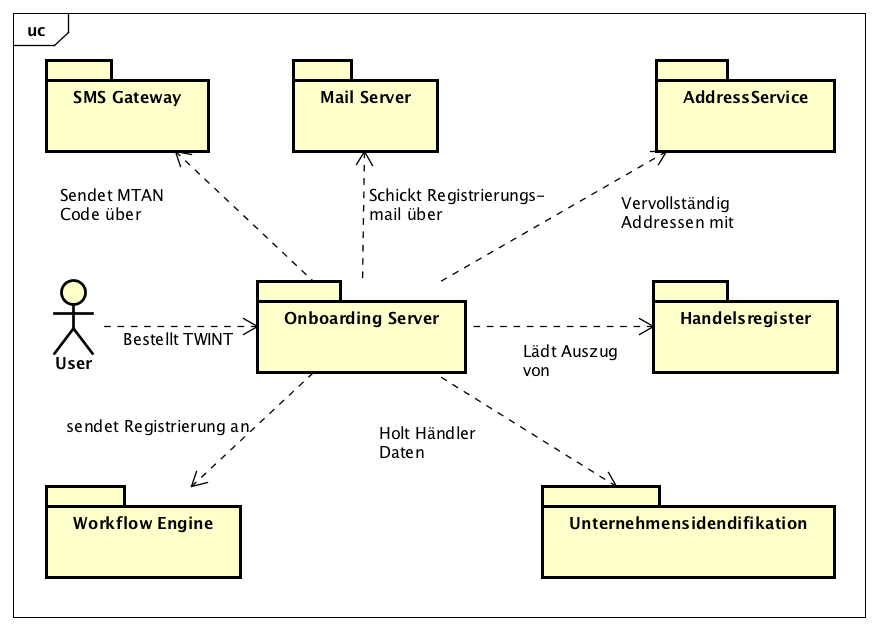
\includegraphics[scale=0.6]{Contextdiagramm.png}
\end{center}

\section{Technischer Kontext}

Die Applikation MEON basiert auf Spring Boot für den Onboarding Server, AngularJS als Frontend sowie Camunda als Workflow Engine. Die Anwendung wird mittels der Container Technologie Docker auf der OpenShift Plattform ausgerollt. 

\section{Externe Schnittstellen}

\subsection{UID Schnittstelle}

\begin{table}[H]
	\centering
	\caption{UID-Schnittstelle}
	\begin{tabular}{ | p{4cm} | p{11cm} | }
		\toprule
		{\textbf{Name}} & {\textbf{Beschreibung}} \\
		\midrule
		Identifikation & URL\\ \hline
		Bereitgestellte Resource & Erlaubt das Abfragen von Unternehmensdaten anhand der Unternehmesidentifikationsnummer. \\ \hline
		Fehlerszenarien & Ist die Schnittstelle nicht verfügbar, muss der Händler die Daten selber eingeben welche falsch sein könntne.\\ \hline
		Qualitätseigenschaften & Maximal 20 Anfragen pro Minuten sonst wird der sender geblockt.  Gartantierte Verfügbarkeit von 362 Tagen \url{https://www.isb.admin.ch/isb/de/home/e-services-bund/services/uid-webservice.html}\\ \hline
		Entwurfsentscheidungen & Falls die Schnittstelle nicht verfügbat ist, werden die Buttons im User Interface ausgeblendet.\\
		\bottomrule
	\end{tabular}
\end{table}

Siehe Spezifikation im Anhang.

\subsection{ZEFIX Schnittstelle}

\begin{table}[H]
	\centering
	\caption{ZEFIX-Schnittstelle}
	\begin{tabular}{  | p{4cm} | p{11cm} | }
		\toprule
		{\textbf{Name}} & {\textbf{Beschreibung}} \\
		\midrule
		Identifikation & URL\\ \hline
		Bereitgestellte Resource & Abfrage des Handelsregisterauszugs \\ \hline
		Fehlerszenarien & Ist die Schnittstelle nicht verfügbar, muss der Hänlder den Auszugs selber hochladen.\\ \hline
		Entwurfsentscheidungen & Falls die Schnittstelle nicht verfügbat ist, werden die Buttons im User Interface ausgeblendet.\\
		\bottomrule
	\end{tabular}
\end{table}

Siehe Spezifikation im Anhang.

\subsection{Adressen Schnittstelle}

\begin{table}[H]
	\centering
	\caption{Address-Schnittstelle}
	\begin{tabular}{  | p{4cm} | p{11cm} |}
		\toprule
		{\textbf{Name}} & {\textbf{Beschreibung}} \\
		\midrule
		Identifikation & URL\\ \hline
		Bereitgestellte Resource & Plz/Ort und Strasse für die Autovervollständigung im XML Format \\ \hline
		Fehlerszenarien & Ist die Schnittstelle nicht verfügbar, muss der Hänlder die Addressdaten selber eingeben.\\ \hline
		Entwurfsentscheidungen & Falls die Schnittstelle nicht verfügbat ist, werden die Buttons im User Interface ausgeblendet.\\
		\bottomrule
	\end{tabular}
\end{table}

Siehe Dokument 'Benutzerhandbuch-Adresschecker-online-V4.pdf' im Anhang.

\subsection{Mail Schnittstelle}

\begin{table}[H]
	\centering
	\caption{Mail-Schnittstelle}
	\begin{tabular}{ | p{4cm} | p{11cm} |}
		\toprule
		{\textbf{Name}} & {\textbf{Beschreibung}} \\
		\midrule
		Identifikation & URL\\ \hline
		Bereitgestellte Resource & Versenden von E-Mails\\ \hline
		Fehlerszenarien & Server nicht erreichbar, wodurch die Mail später nochmals gesendet werden muss.\\ \hline
		Entwurfsentscheidungen & Falls die Schnittstelle nicht verfügbat ist, werden die Buttons im User Interface ausgeblendet.\\
		\bottomrule
	\end{tabular}
\end{table}

\subsection{ATMS Schnittstelle}

\begin{table}[H]
	\centering
	\caption{ATMS-Schnittstelle}
	\begin{tabular}{ | p{4cm} | p{11cm} | }
		\toprule
		{\textbf{Name}} & {\textbf{Beschreibung}} \\
		\midrule
		Identifikation & URL\\ \hline
		Bereitgestellte Resource & Versenden von E-Mails\\ \hline
		Fehlerszenarien & Server nicht erreichbar, wodurch die Mail später nochmals gesendet werden muss.\\ \hline
		Entwurfsentscheidungen & Falls die Schnittstelle nicht verfügbat ist, werden die Buttons im User Interface ausgeblendet.\\
		\bottomrule
	\end{tabular}
\end{table}
